\section{Durchführung und Auswertung}

\subsection{LABVIEW-Messprogramm}

Wir haben zur Messung das bereits vorhandene Messprogramm verwendet. Allerdings zeigte sich im Laufe der Messungen, dass die Qualität gesteigert werden kann, wenn zwischen den einzelnen Messungen die Hochspannung auf $0V$ heruntergefahren wird. Durch das Methan können dann verbleibende Ionen herausgespült werden. Daher haben wir das Programm um diese "`Reinigungsphase"' erweitert.

\subsection{Zählrohrcharacteristik}

Wir haben damit begonnen, die Zählrohrcharakteristik aufzunehmen. Dazu haben wir eine \atom{238}{}{U} Probe verwendet, die eine gute Zählrate zeigt.

\begin{figure}[H]
 \centering 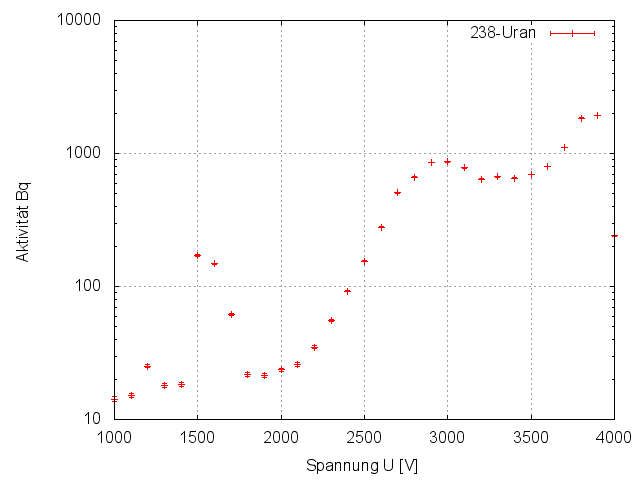
\includegraphics[width=0.9\linewidth]{Messwerte/plots/U238.png}
 \caption{Zählrohrcharakteristik, gemessen mit \atom{238}{}{U}}
\end{figure}

Der Graph zeigt den erwarteten Verlauf, abgesehen von einigen Ausreisern am Anfang des $\alpha$-Plateaus. \atom{238}{}{U} zerfällt durch $\alpha$-Zerfall in \atom{234}{}{Th} (Thorium). Dieses zerfällt mit einer Halbwertszeit $T_{1/2} = 24.10d$ durch einen $\beta^-$-Zerfall in \atom{234}{}{Pa} (Proactinium), welches ebenfalls durch $\beta^-$-Zerfall in \atom{234}{}{U} zerfällt. Deshalb sehen wir in der Zählrohrcharakteristik sowohl ein Plateaubereich, in dem haupsächlich $\alpha$-Strahlung detektiert wird bei ca. $U = 1200V$ bis $U = 2200V$ als auch einen Plateaubereich in dem $\alpha$- und $\beta$-Strahlung detektiert werden zwischen $2800V$ und $3500V$.

Auf das Abziehen des Untergrundes haben wir verzichtet, einerseits da der Untergrund eine Aktivität von ca. $0.001Bq$ bis maximal $1.0Bq$ zeigte, also deutlich weniger als die eigentliche Intensität. Andererseits sind die Ergebnisse der Untergrundmessung eh fraglich, wie später erleutert wird.

\subsection{Bestimmung der Halbwertszeit von \atom{147}{}{Sm} ($\alpha$-Zerfall)}

Wir haben für den im voherigen Versuchsabschnitt ermittelten $\alpha$-Plateaubereich eine grobe Messung mit einer \atom{147}{}{Sm}-Probe vorgenommen. 

\begin{figure}[H]
 \centering 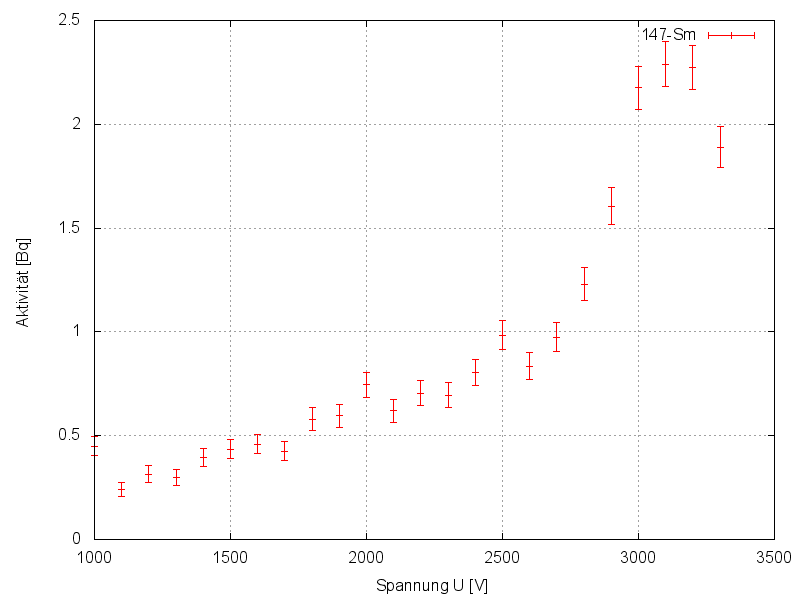
\includegraphics[width=0.9\linewidth]{Messwerte/plots/Sm147_plateau.png}
 \caption{Plateaubereich, gemessen mit \atom{147}{}{Sm}}
\end{figure}